\documentclass{article}
\usepackage{tikz}    
\usepackage[final,nonatbib]{nips_2016}

\usepackage[utf8]{inputenc} % allow utf-8 input
\usepackage[T1]{fontenc}    % use 8-bit T1 fonts
\usepackage{hyperref}       % hyperlinks
\usepackage{url}            % simple URL typesetting
\usepackage{booktabs}       % professional-quality tables
\usepackage{amsmath}       
\usepackage{caption}       
\usepackage{subcaption}       
\usepackage{amsfonts}       % blackboard math symbols
\usepackage{nicefrac}       % compact symbols for 1/2, etc.
\usepackage{microtype}      % microtypography

\usepackage[backend=bibtex]{biblatex}
\bibliography{smallbiblio}
%\usetikzlibrary{arrows}
\tikzset{>=latex}
%\usetikzlibrary{arrows.meta}

\title{Backpropagation of Hebbian plasticity for lifelong learning}

\author{
    Thomas Miconi\\
    The Neurosciences Institute\\
    La Jolla, CA, USA\\
    \texttt{miconi@nsi.edu}
}

\begin{document}

\maketitle

\begin{abstract}
Hebbian plasticity allows biological agents to learn from their lifetime
experience, extending the fixed information provided by evolutionary search.
Conversely, backpropagation methods can build high-performance fixed-weights
networks, but are not currently equipped to design networks with Hebbian
connections. Here we use backpropagation to train fully-differentiable plastic networks, such that
backpropagation determines not only the baseline weights, but also the
plasticity of each connection. To perform this backpropagation of Hebbian
plasticity (BOHP), we derive error gradients for neural networks with Hebbian
plastic connections. The equations for these gradients turn out to follow a
simple, recursive form. We apply this method to train small networks for simple
learning tasks inspired from classical conditioning. We show that, through
Hebbian plasticity, the networks perform fast learning of
unpredictable environmental features during their lifetime, successfully solving
a task that fixed-weight feedforward networks cannot possibly solve. We conclude that
backpropagation of Hebbian plasticity offers a powerful model for lifelong
learning.
\end{abstract}


\section{Introduction}

Living organisms endowed with neural systems show remarkably complex behaviors.
While much of this complexity results from evolutionary learning over millions
of years, it also results from the ability of neural systems to learn from
experience. Lifetime learning is beneficial for several reasons. For one thing,
some environmental features can simply not be predicted at birth (e.g. the
position of food sources, the identifying features of other individuals for
social species, etc.), requiring learning from experience in contact with the
environment. Furthermore, even for predictable environmental features, much of
the information necessary to produce adaptive behavior can be obtained ``for
free'' by learning from the environment, thus removing a potentially huge chunk
of the search space that evolution must explore. For example, the connectivity
of primary visual cortex is fashioned by Hebbian plasticity rather than having
each single connection genetically specified, allowing a huge number of cells
to organize into a powerful, reliable information-processing system with
minimal genetic specification.

Lifetime long-term learning in living brains occurs through some
form of synaptic plasticity. While synaptic plasticity is complex and still not
fully understood, a significant component of this process seems to follow the Hebbian principle: a
cell that consistently contributes in making another cell fire will build a
stronger connection to that cell. Note that this generic principle can be
implemented in many different ways, including covariance learning, instar and
outstar rules, BCM learning, etc. (see \cite{Vasilkoski2011-ww} and references therein). 

Backpropagation methods can train neural networks to perform remarkably complex
tasks. However, they are generally applied to fixed-weights networks. Several
methods have been proposed to make lifelong learning amenable to
backpropagation, including most recently neural Turing machines
\cite{Graves2014-ch,Santoro2016-jn} and
memory networks \cite{Sukhbaatar2015-ly}. However, it would be useful to incorporate the powerful, well-studied
principle of Hebbian plasticity in backpropagation
training.

Here we show that neural networks with Hebbian synapses can be optimized by
gradient descent and backpropagation. To this end, we derive analytic
expressions for the gradients of neural responses
over weights and plasticity parameters. Finally, we use these gradients to train neural
networks for simple conditioning tasks, showing that the resulting networks
successfully learn from experience.

All software used for the present paper is available at
\texttt{http://github.com/thomasmiconi}.

\section{Networks with Hebbian synapses}

We consider networks where the strength of each connection can vary according to
Hebbian plasticity over the course of each network's ``lifetime'', or
\emph{episode}. We will arrange things so that each network is fully specified
by fixed parameters which determine both the baseline weight \emph{and} the degree of plasticity of each connection.
These parameters are fixed and unchanging over an episode, but govern the way in which
each connection changes over the course of an episode due to Hebbian plasticity. At the end of each
episode (or minibatch of episodes) we want to apply backpropagation to optimize
these networks parameters. Therefore, our goal is to find expressions for the gradient of the response of any
given cell, over the weights and plasticity parameters of its incoming connections.

Note that these gradients will take a time-dependent form: when Hebbian
plasticity is present, the activity of a cell at a given time can influence its
future responses over the rest of the episode, even in the absence of recurrent
connections, due to its Hebbian effect on the long-term connection weight. 

To model Hebbian plasticity, we maintain a time-dependent quantity for each
connection in the network, which we call the \emph{Hebbian trace} for this connection.
This quantity is simply the running average of the product of pre- and
post-synaptic activities.
Thus, for a given target cell, the Hebbian trace associated with its $k$-th incoming
connection is defined as follows:

\begin{equation}
\label{eq:hebb}
Hebb_k(t) = (1-\gamma) * Hebb_k(t-1) + \gamma * x_k(t) * y(t)
\end{equation}

where $y(t)$ is the activity of the post-synaptic cell, $x_k(t)$ is the activity
of the pre-synaptic cell, and $\gamma$ is a time constant. While other
expressions of Hebbian plasticity are possible, this simple form turns out to be
adequate for our present purposes.

The Hebbian trace is maintained automatically, independently of network
parameters, for each connection. Given this Hebbian trace, the
actual strength of the connection at time $t$ is determined by two fixed parameters: a fixed
weight $w_k$, which determines the ``baseline'', unchanging component of the
connection; and a \emph{plasticity parameter} $\alpha_k$, which specifies how
much the Hebbian trace influences the actual connection. More formally, the
response $y$ of a given cell can be written as a function of its inputs as
follows:

\begin{equation}
\label{eq:y}
y(t) = \tanh\left\{\sum_{k \in inputs}[w_k x_k(t) + \alpha_k Hebb_k(t) x_k(t)] +
b\right\}
\end{equation}


Where $b$ is a bias parameter. 


\section{Gradients}

In order to use backpropagation, we must find the gradient of $y$ over the $w_k$ and
$\alpha_k$ parameters. As mentioned above, these gradients will necessarily
involve activities at previous times. Fortunately, these gradients turn out to
have a simple, recursive form. 

Temporarily omitting the $\tanh$ nonlinearity (see below), we get the
following expressions: 

\begin{equation}
\label{eq:gradw}
\frac{\partial y(t_z)}{\partial w_k} = x_k(t_z) + \sum_{l \in inputs}[\alpha_l
x_l(t_z) \sum_{t_u<t_z}(1-\gamma) \gamma^{t_z-t_u} x_l(t_u) \frac{\partial
y(t_u)}{\partial w_k}]
\end{equation}

\begin{equation}
\label{eq:gradalpha}
\frac{\partial y(t_z)}{\partial \alpha_k} = x_k(t_z) Hebb_k(t_z) + \sum_{l \in inputs}
[\alpha_l x_l(t_z) \sum_{t_u<t_z}(1-\gamma) \gamma^{t_z-t_u} x_l(t_u) \frac{\partial
y(t_u)}{\partial \alpha_k}]
\end{equation}

(See Appendix for a full derivation.)

These equations express the gradient of $y(t_z)$ as a function of the gradients
of $y(t_z<t_u)$, that is, recursively.

In each of these equations, the summand over previous times $t_u<t_z$ is
essentially the partial derivative of the Hebbian traces at time $t_{z}$
with respect to either $w_k$ (Eq. \ref{eq:gradw}) or $\alpha_k$ (Eq.
\ref{eq:gradalpha}). Since the Hebbian trace is the exponential average of
previous products of $x$ and $y$, these partial derivatives turn out to be
sums of the previous gradients of $y$ over the corresponding parameter,
multiplied by the concomitant activity of the input cell $x_k$ (the $\gamma$ terms
account for the exponential decay of the running average). Thus, the gradient at
time $t_z$ is a function of (the weighted sum of) the gradients at times
$t_u<t_z$.

Note that the sum is over the Hebbian traces of \emph{all} inputs to $y$, not just the
one associated with connection $k$ for which we are computing the gradient. This is because the values of $w_k$ and
$\alpha_k$, by affecting $y$, also influence the Hebbian traces of all other
connections to $y$. This effect must be accounted for in the above gradients.

The above expression omits the $\tanh$ nonlinearity: it really provides the
gradient of the expression within the curly braces in Eq. \ref{eq:y}, that is,
the ``raw'' output (call it $y_{raw}$) provided by incoming excitation and biases. To obtain
the full gradient $\frac{\partial y(t_z)}{\partial w_k}$, we simply rewrite $y$ as $y =
\tanh(y_{raw})$ and apply the chain rule: $\frac{\partial y}{\partial w_k} =
\frac{\partial \tanh(y_{raw})}{\partial y_{raw}} \frac{\partial y_{raw}}{\partial
w_k} = (1 - y^2)\frac{\partial y_{raw}}{\partial w_k}$, where $\frac{\partial
y_{raw}}{\partial w_k}$ is provided by Eq. \ref{eq:gradw} above (and similarly
for $\frac{\partial
y_{raw})}{\partial \alpha_k}$ 

\section{Experiments}

\subsection{Task}

To test the BOHP method, we train networks to perform a simple task inspired by
classical conditioning \cite{Fanselow2016-gz}. In this task, at every time step, the network can encounter two kinds of
stimulus, one of which has a certain probability of being associated with a
``pain'' signal. Which stimulus predicts the potential presence of pain 
changes unpredictably from one episode to the next, but remains stable during each
episode.  For each episode, the network's task is to learn which of
the two stimuli is
potentially pain-causing, and produce high response (``fear'') whenever
this stimulus is present, even in the absence of pain. 

The networks have access to three sensors, one for each stimulus (S1 and S2),
and one for the pain signal (P). At any time step within the episode, one or
both stimuli may be present, setting the associated stimulus sensor to 1; also,
a pain signal may be delivered, setting the P sensor to 1. The P sensor is
activated with probability .3 when the pain-associated stimulus is present, and
never activated otherwise (P sensor activation is independent of the presence or
absence of the other, non-associated stimulus). We expect the network to
produce output 1 when the pain-associated stimulus is present (even if no pain
is currently delivered), and 0 otherwise.

The error for each timestep is simply the squared difference between expected
and actual output. Each episode lasts 100 timesteps. Note that we do not take
into account error during the first 20 timesteps (the ``learning period'' for
each episode). While not strictly necessary, we found that allowing for a
``free'' exploratory learning period improved learning. Note that
backpropagation will not seek to reduce error during the learning period, but
will still take into account network activity during the learning period to
reduce the error after the learning period, as expressed by the recursive
gradients in Eqs. \ref{eq:gradw} and \ref{eq:gradalpha}.

\subsection{Results}

\begin{figure}
\centering
\begin{subfigure}[t]{0.4\textwidth}
\centering
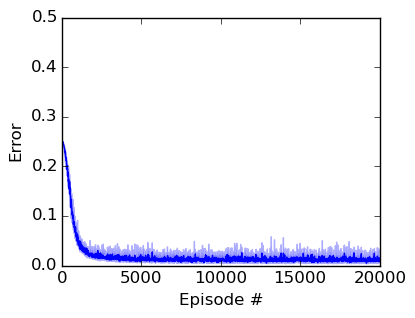
\includegraphics[scale=0.5]{figexcl.png}
\subcaption{Mutually exclusive stimuli}
\end{subfigure}
\begin{subfigure}[t]{0.4\textwidth}
\centering
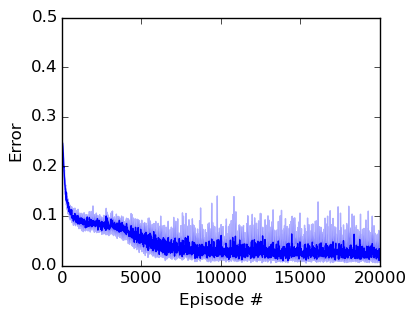
\includegraphics[scale=0.5]{figuncorr.png}
\subcaption{Uncorrelated stimuli}
\end{subfigure}
\caption{Mean absolute error per timestep over each episode, for mutually
exclusive stimuli (a) and uncorrelated stimuli (b). Dark lines indicate median
over 20 runs, while shaded areas indicate interquartile range.}
\label{fig:error}
\end{figure}


We first use a version of the task in which the two stimuli are mutually
exclusive: only one of S1 or S2 can be active at any given time step. In this
setting, the ``fearful'' stimulus (the one that the network should learn to
detect and respond to) is the only one that can be active when the
pain sensor is also active, which should facilitate learning. 
For this simple version of the task, we use very simple networks consisting of one layer of weights, with a single
output cell directly connected to each sensor. 

We find that BOHP easily solves this task, designing networks that learn to
associate incoming stimuli with the presence or absence of the pain signal (see
Figure \ref{fig:error}a). The
resulting networks consistently follow the same pattern (Figure
\ref{fig:networks}a). The P sensor sends a
very strong, fixed-weight connection to the output cell. As a result, the output
cell $y$ is activated whenever the pain signal is present, as expected. By contrast, the
connections from the two stimulus
sensors have nearly zero fixed weight $w$, but very high plasticity $\alpha$. As
a result, S1 and S2 initially provide zero excitation to the  output cell $y$;
however, as soon as one of S1 or S2 is activated at the same time as P, it will
immediately produce a large Hebbian trace for its connection to $y$ (since $y$
will be activated by the P sensor, and Hebbian traces accumulate the product of
input and output for each connection). Because of the high $\alpha$, this high
Hebbian trace will immediately create a strong overall connection from the
active stimulus sensor to $y$. As a result, this sensor can now activate $y$ on
its own, even in the absence of pain, exhibiting successful conditioning.

We then slightly modify the task by making the two stimuli uncorrelated: the
presence or absence of one stimulus is independent of the other (but only one of
these is potentially associated with pain). As a result, the non-predictive
stimulus can now be active at the same time as the P sensor, making the previous
strategy ineffective since it would result in having non-zero response to the
non-predictive stimulus. 

We find that BOHP cannot solve this problem with simple one-layer networks over
a wide range of parameters. We therefore expand the networks in the most minimal
way possible, by adding a hidden layer with two hidden neurons H1 and H2. Only the connections between input and
hidden neurons can be plastic; the hidden-to-output connections can only have
fixed weights.

With such two-layer networks, BOHP again easily solves the task (Figure
\ref{fig:error}b), with a somewhat different solution (Figure
\ref{fig:networks}b). Each of the two hidden neuron still receives a strong
fixed connection from the $P$ sensor, making both of them active whenever P is.
However, they now receive opposite-sign plastic connections with from the
stimulus sensors: one of the hidden units has high positive $\alpha$ from S1
and high \emph{negative} $\alpha$ from S2, and vice-versa for the other hidden
unit.  Furthermore, both hidden units have large negative biases, making them
inactive unless they receive high excitation.  We propose the following
interpretation. Notice that the Hebbian trace for the predictive stimulus will
be much larger than for the non-predictive stimulus.  Suppose that S1 is the
associated stimulus. As a result, one hidden unit (label it H1) will have
strong positive connection from S1 (due to the high Hebbian trace between S1
and hidden neurons), but also a weak inhibitory connection from S2 (due to the
weak Hebbian trace between S2 and hidden neurons), making it active whenever S1
is present (even if S2 is present) and inactive otherwise. By contrast, the
other unit (H2) will have a strong inhibitory connection from S1, and weak
excitatory connection from S2, making it inactive at any time. If S2 is the
predictive stimuli, then the roles are reversed: H1 is never active, and H2 is
only active when S2 is present. Thus, H1 and H2 jointly detect the predictive
stimulus (whichever it is) and remain quiescent otherwise (``quiescent'' here
means negative output, which is compensated by a positive bias on the single
neuron of the output layer).

% An additional factor is that the negative alpha will reduce the magnitude of
% the Hebbian trace, since it will create a negative correlation between the
% input and output! This is an extension of the general idea that Hebbian
% plasticity is fundamentally self-reinforcing...




\begin{figure}
\centering
%\includegraphics[scale=0.25]{figgraphs.png}
% Actual code for the graphs (be sure to uncomment \usepackage{tikz} in the header).  
\begin{subfigure}[t]{0.2\textwidth}
\centering
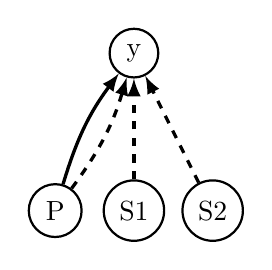
\begin{tikzpicture}
\begin{scope}[every node/.style={circle,thick,draw}]
\node (y) at (1,2) {y};
\node (P) at (0,0) {P};
\node (S1) at (1,0) {S1};
\node (S2) at (2,0) {S2};
\end{scope}
%\begin{scope}[>={Stealth[black]},
\begin{scope}[
        every node/.style={fill=white,circle},
    every edge/.style={draw=black,very thick}]

    \path [->] (P) edge   [bend left=10](y);
    \path [dashed][->] (P) edge   [bend right=10](y);

    %\path [->] (S2) edge  [bend left=10](y);
    \path [dashed][->] (S2) edge  (y);

    %\path [->] (S1) edge [bend left=10] (y); 
    \path [dashed][->] (S1) edge  (y); 

\end{scope}
\end{tikzpicture}
\subcaption{Solution for mutually exclusive stimuli}
\end{subfigure}
\qquad
\begin{subfigure}[t]{0.35\textwidth}
\centering
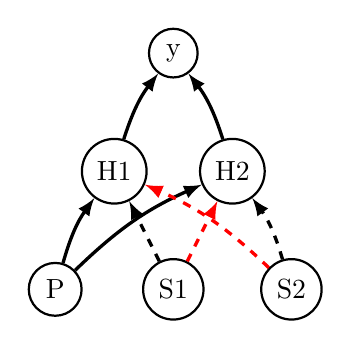
\begin{tikzpicture}
\centering
\begin{scope}[every node/.style={circle,thick,draw}]
\node (y) at (1.5,3) {y};
\node (H1) at (.75,1.5) {H1};
\node (H2) at (2.25,1.5) {H2};
\node (P) at (0,0) {P};
\node (S1) at (1.5,0) {S1};
\node (S2) at (3,0) {S2};
%\node (D) at (2.5,1) {D};
%\node (E) at (2.5,-3) {E};
%\node (F) at (5,3) {F} ;
\end{scope}
\begin{scope}[%>={Stealth},
        every node/.style={fill=white,circle},
    every edge/.style={draw=black,very thick}]
    
    \path [->] (P) edge   [bend left=10](H1);
    \path [->] (P) edge   [bend left=10](H2);

    %\path [->] (S2) edge  [bend left=10](y);
    \path [dashed][->] (S1) edge  (H1);
    \path [dashed][->] (S1) edge [red] (H2);

    %\path [->] (S1) edge [bend left=10] (y); 
    \path [dashed][->] (S2) edge [red,bend right=10](H1); 
    \path [dashed][->] (S2) edge  [bend right=10](H2); 

    \path [->] (H1) edge   [bend left=10](y);
    \path [->] (H2) edge   [bend right=10](y);


    %\path [->] (E) edge node {$8$} (F); 
    %\path [->] (B) edge[bend right=60] node {$1$} (E); 
\end{scope}
\end{tikzpicture}
\subcaption{Solution for uncorrelated stimuli}
\end{subfigure}
%\qquad
%\begin{subfigure}[t]{0.3\textwidth}
%\parbox[t]{4cm}{
%\parbox[t][][t]{0.9\textwidth}{
\begin{minipage}[b]{0.35\textwidth}
\centering
\begin{itemize}
\item[]\tikz{\path[very thick,->,draw=black] %,>={Stealth}] 
        (0,0) -- (1,0) ;}Excitatory fixed-weight connection
\item[]\tikz{\path[very thick,->,draw=red] %,>={Stealth}] 
        (0,0) -- (1,0) ;}Inhibitory fixed-weight connection
\item[]\tikz{\path[very thick,->,dashed,draw=black] %,>={Stealth}] 
        (0,0) -- (1,0) ;}Excitatory plastic connection
\item[]\tikz{\path[very thick,->,dashed,draw=red] %,>={Stealth}] 
        (0,0) -- (1,0) ;}Inhibitory plastic connection
\end{itemize}
\end{minipage}
%%\end{subfigure}
%%%% Look at 'example of perrin jablonski diagram' for how to make a legend with itemize...

\caption{Schematic networks found by BOHP to solve the conditioning problem with
mutually exclusive stimuli (a) or uncorrelated stimuli (b).}
\label{fig:networks}
\end{figure}


\section{Conclusions and future work}


In this paper we have introduced a method for designing networks endowed with
Hebbian plasticity through gradient descent and backpropagation. To this end, we
derived gradients of neural activities over input weights and plasticity
parameters. The method successfully solved a simple conditioning task, learning
to detect and respond to a conditioned stimulus.

Here we only use a very simple form of Hebbian plasticity, namely, the
running average of the product between pre- and post-synaptic activities.
However, there are other possible formulations of Hebbian plasticity, such as
covariance learning (mean-centering pre- and post-synaptic responses), instar
and outstar rules, or BCM learning. These can be implemented in BOHP by updating
the gradient equations appropriately, which might expand the capacities of BOHP. However, as shown above, the simple
Hebbian plasticity used here can already produce fast, reliable lifetime
learning.

In addition, while we used very simple networks with only one plastic layer, the gradients
derived here can potentially be applied to more complex networks, including large
multi-layer networks and recurrent networks. 
We are currently exploring the application of BOHP to larger networks for more complex tasks.

In conclusion, we suggest that backpropagation of Hebbian plasticity is an
efficient 
way to endow neural networks with lifelong learning abilities, while still being
amenable to gradient descent. 

\section*{Appendix}

Here we provide a more complete derivation of the gradients of output cell
response $y$ at a given timestep $t_z$ with regard to the $\alpha$ coefficient
of an incoming connection $k$ (where input activity of the pre-synaptic neuron
at this connection is denoted by $x_k$). 

First we simply write out the
full expression for $y$, from Equation \ref{eq:y} (again, note that we omit
the $\tanh$ nonlinearity):

\[
\frac{\partial y(t_z)}{\partial \alpha_k} = \frac{\partial }{\partial \alpha_k}[ \sum_{l \in inputs}w_l x_l(t_z) + \sum_{l \in inputs}\alpha_l Hebb_l(t_z) x_l(t_z) ] 
\]

The first summand on the right-hand side denotes the inputs to $y$ from incoming connections through the fixed weights; since this term does not depend on $\alpha$ in any way, we can remove it from the gradient computation.

The second summand denotes inputs through plastic connections. The cases for
$l=k$ and $l\neq k$ must be handled differently, since we are differentiating
with regard to $\alpha_k$:

\begin{align}
\frac{\partial y(t_z)}{\partial \alpha_k} &= \frac{\partial }{\partial \alpha_k}[
\sum_{l \neq k }\alpha_l Hebb_l(t_z) x_l(t_z) + \alpha_k Hebb_k(t_z) x_k(t_z)]\\
&= \sum_{l \neq k }[\frac{\partial }{\partial \alpha_k} (\alpha_l x_l(t_z) Hebb_l(t_z))] + \frac{\partial }{\partial \alpha_k}[\alpha_k Hebb_k(t_z) x_k(t_z)]
\end{align}

With regard to $\alpha_k$, the derivative in the first right-hand-side term has the
form $d(Const*f(\alpha_k))/d\alpha_k$, since only the $Hebb_l(t_z)$ depends on $\alpha_k$
(indirectly through $y$). By contrast, the second right-hand-side term has the
form $d(Const*\alpha_k*f(\alpha_k))/d\alpha_k$, so we must develop it using the identity
$(xf(x))'=xf'(x)+f(x)$. Therefore:

\[
\frac{\partial y(t_z)}{\partial \alpha_k} = \sum_{l \neq k }[\alpha_l
x_l(t_z)\frac{\partial }{\partial \alpha_k}Hebb_l(t_z)] +
x_k(t_z)(\alpha_k\frac{\partial }{\partial \alpha_k}Hebb_k(t_z) + Hebb_k(t_z))
\]

Replacing the $Hebb(t)$ terms by their full expression as the accumulated product of $x$ and
$y$ (Eq. \ref{eq:hebb}), we get:

\begin{align}
\frac{\partial y(t_z)}{\partial \alpha_k} &= \sum_{l \neq k }[\alpha_l x_l(t_z) \frac{\partial }{\partial
\alpha_k}\sum_{t_u < t_z}(1-\gamma)\gamma^{tz-tu}x_l(t_u)y(t_u))] \nonumber \\ 
& \qquad {} + x_k(t_z)[\alpha_k\frac{\partial}{\partial \alpha_k}\sum_{t_u <
t_z}(1-\gamma)\gamma^{tz-tu}x_k(t_u)y(t_u) + Hebb_k(tz)]\\
&= \sum_{l \neq k }[\alpha_l x_l(t_z) \sum_{t_u < t_z}(1-\gamma)\gamma^{tz-tu}x_l(t_u)\frac{\partial }{\partial
\alpha_k}y(t_u)] \nonumber \\
& \qquad {} + x_k(t_z)[\alpha_k\sum_{t_u <
t_z}x_k(t_u)(1-\gamma)\gamma^{tz-tu}\frac{\partial}{\partial \alpha_k}y(t_u) + Hebb_k(tz)]\\
&= \sum_{l \in inputs}[\alpha_l x_l(t_z)\sum_{t_u <
t_z}(1-\gamma)\gamma^{t_z-t_u}x_l(t_u)\frac{\partial
}{\partial
\alpha_k}y(t_u)] +
x_k(t_z)Hebb_k(tz)
\end{align}


where in the last equation above, $l$ runs over all incoming connections to $y$,
including $k$. This recursive gradient equation is identical to Eq.
\ref{eq:gradalpha}.

Eq. \ref{eq:gradw} is derived much in the same manner (though slightly simpler
since we do not need to use the $(xf(x))'=xf'(x)+f(x)$ identity). For future applications to
many-layers networks, equations for the gradient
$\frac{\partial y(t_z)}{\partial x_k}$ are easily obtained with a similar
derivation.

\small
\printbibliography

\end{document}

